\documentclass[12pt]{article}
\usepackage[top=1.00in, bottom=1.0in, left=1.1in, right=1.1in]{geometry}
\renewcommand{\baselinestretch}{1.1}
\usepackage{graphicx}
\usepackage{natbib}
\usepackage{amsmath}
\bibliographystyle{..//sub_projs/refs/styles/besjournals.bst}
\def\labelitemi{--}
\parindent=24pt
\title{Do hysteranthous tree species invest less in pollinator attraction than seranthous species? A basic test of the pollinator visability and water limitation hypotheses}
\begin{document}
\maketitle



\section{Introduction}
Why do some species of deciduous woody species flower before their leaves emerge (hysteranthy)? There seem to be lots of drawbacks. This phenological condition is risky, putting flowers at greater risk to damage from late season frost-- While leave can reflush if damaged you flowers tend not to.\\

It is also a substantial resource investment from stored carbohydrates at a time of year when these resources are at their lowest levels. There must be some adaptive tradeoff/benefit to hysteranthy.\\

My work and others have shown that wind pollination efficiency appears to select for hysteranthy (pollen transfer is not obscured by vegetative structures). However, this fails to explain hysteranthy in insect pollinated taxa which is not uncommon. For example, I found that 25 out of the 44 species of North American \emph{Prunus} species are hysteranthous.

\citet{Janzen1967} suggests that this adaptation may be to increase pollinator visibility, but this has not be widely tested. This is rather difficult to test, because a pollination syndrome is a suite of traits, and macro-evolutionary differences amoung even closely related species may compinsate for each other...for example a synanthous species might make bigger or smellier flower displays than a hysteranous sister sp., so you wouldn't see a difference in attraction in real timeif you spent all your time following bee around.\\

Alternatively hysteranthy could might be an adaptation for dry enviroments. Yet again, there are a suite of traits that could determine drought tolerance.\\ 

However, the same co-evolved traits that could obscure ecological comparisons between hysteranthous synthanthous congeners could be the finger prints of selection.\\

Some tradeoffs about floral displays to condsider:
\begin{enumerate}
\item Larger dispays (flower size, inflorescence size) increase pollinator visitation \citep{Conner:1996aa,Mitchell:2004aa, Schmid-Hempel:1988aa,Stanton:1988aa, Worley:2000aa}
\item Large floral displays are more costly, especially in dry/stressful environments \citep{Lambrecht:2013aa,Herrera:2009aa,DEBUSSCHE:2004aa}
\end{enumerate}

Hysteranthy could be a strategy that helps both of these things. If flowers are more visible (not obscured by vegetation) they can be smaller. If they have to be small due to physiological/environmental constraints, evolving hysteranthy might be a way to compensate for reduced visibility.\\

Note: There is no way to untangle this ``just so" story, but these hypotheses make predictors about flower size and habitat in hysteranthous species.\\

Prediction:
\begin{enumerate}
\item Flowers or inflorescences of hysteranthous species should be smaller and invest less in chemical attraction than those of their seranthous congeners.
\item Hysteranthous species should be generally found in dryer areas.
\end{enumerate}

These hypotheses could be readily tested by:
\begin{enumerate}
\item Measuring flowers and display size on herbarium specimens or just use eflora information (see below) in hysteranthous and seranthous congeners.
\item Recording locality informaton on said specimens and comparing aridity of those sites. 
\item Collecting flowers from arnold arboretum and doing (or sending to a lab for) volatile analysis.
\end{enumerate}

\section{Preliminary evidence}
Hypothesis 1 has been suggested for a few species in the genus \textit{Cornus} by \citet{Gunatilleke1984}.\\

Additionally I collected mean flower size and flowers/inflorescences data for the 44 \textit{Prunus} and 27 \textit{Rhododendron} species of North America from The Flora of North America. A signal for hypothesis 1 appears to be present in these genera (Fig. \ref{fig:prunus}).

\begin{figure}[h!]
    \centering
 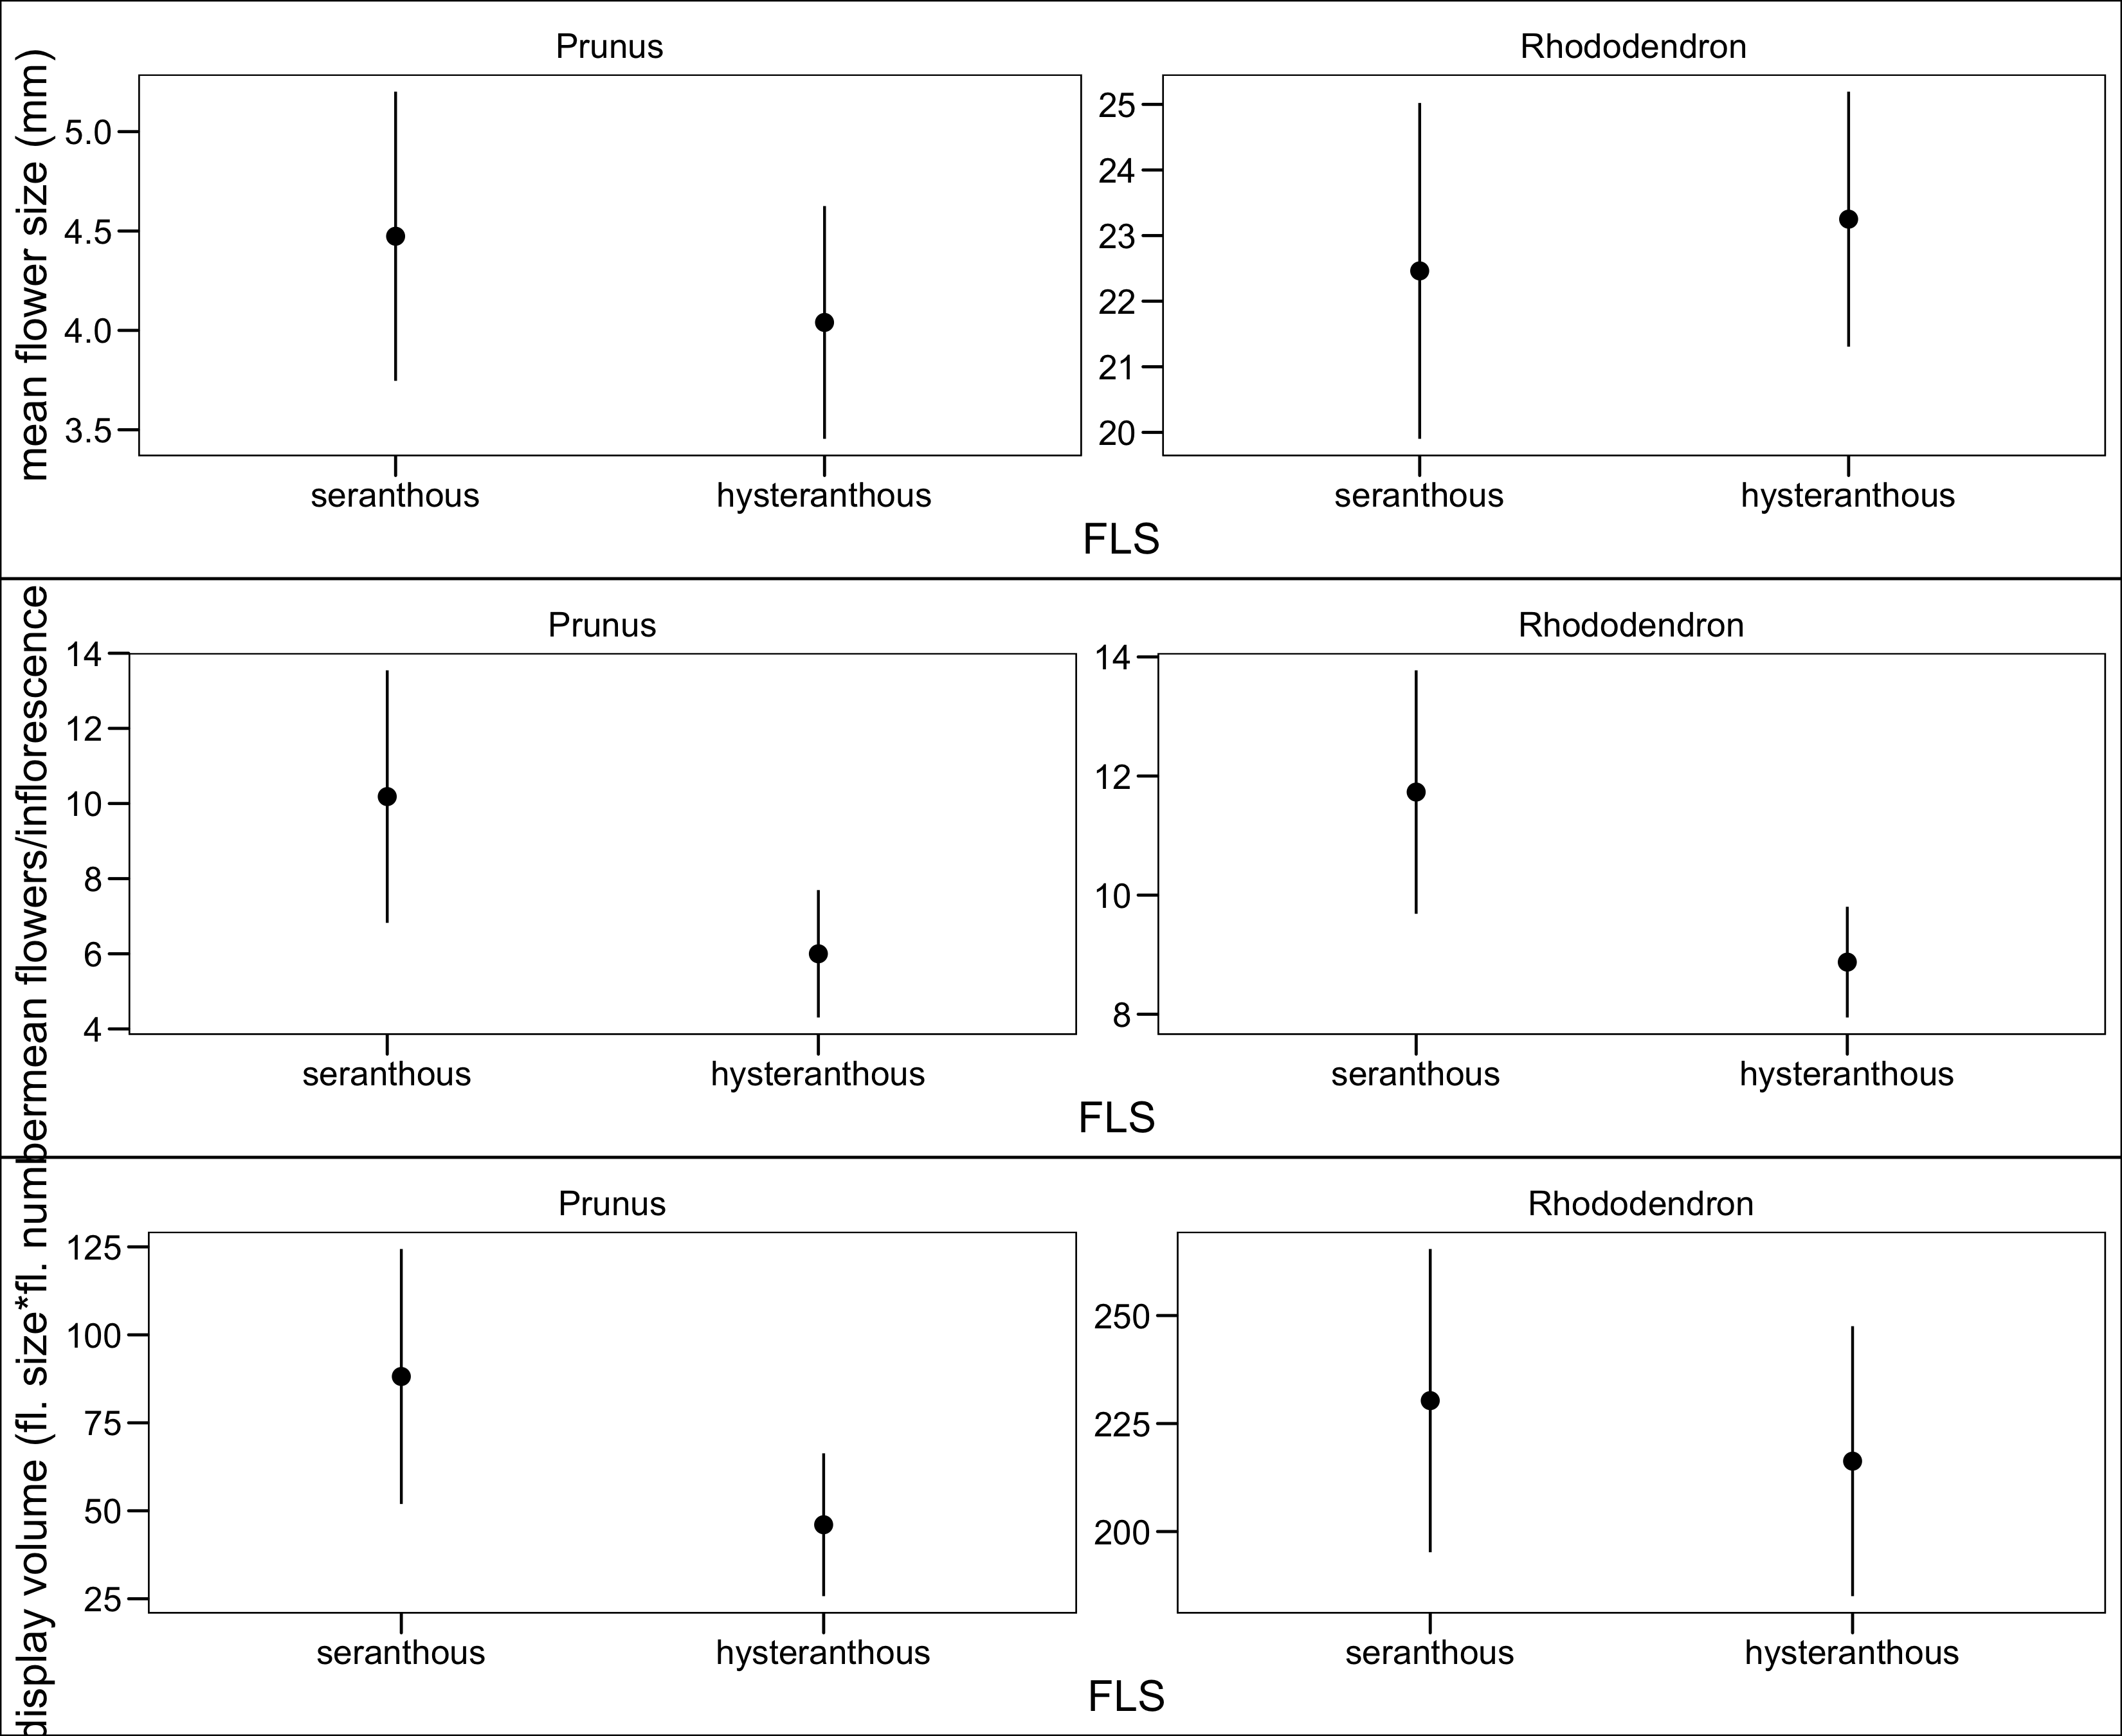
\includegraphics[width=\textwidth]{prelim_plot.png}
    \caption{\textbf{Hysteranthous species in the genera \texit{Rhododendron} and \textit{Prunus} found in North America appear to invest less in their floral displays than their seranthous congeners.} Hysteranthous \textit{Prunus} sps. have smalle flowers, fewer flowers per inflorescences and a smaller floral display (number x size) tha seranthous congeners. Hysteranthous ans seranthous \textit{Rhododendron} have similar average flowers sizes (corolla), but hysteranthous species have fewer flowers per inflorescence, resuling a smaller display on average than seranthous species. } 
    \label{fig:prunus}
\end{figure}

\section{Proposal:}
\subsection{Part 1:}
Using digitized herbarium specimens and Image J, measure the size of flowers and count the number of flowers per inflorescence for hysteranthous and seranthous (biotically-pollinated) congeners.\\
Genera with FLS variation: \emph{Amelanchier, Prunus*, Asimina, Cornus, Rhododendron*, Acer, Magnolia, Dirca, Rhus, Vaccinium, Lindera, Salix}. * indicates complete FLS details in eflora.org, which could allow for a very through treatment of these large genera. Other genera would probably include 2-10 comparisons.\\

Alternatively, I could really dig in on \textit{Prunus}.\\

\subsection{Part 2:} 
This part is optional.\\
Apply for a Deland Award or other arboretum money. In Spring 2021, collect flowers from hysteranthous/non-hysteranthous congeners (~3-5 genera) and quantify the volatiles for attracting pollinators (I'd need to learn alot more about this). Could use many of the same species as Jessica Savage did for her phloem work.

\section{Conclusion:}
This is NOT the pivot to applied climate change ecology I had envisioned. However, it seems likea fairy easy way to put a nice bow on 3 chapters of hysteranthy. It is data I can probably collect for one hour a daym and I expect the analysis (at least of part 1) would be fairly straight forward.

\bibliography{investmentrefs}
\end{document}